\section{Grundlagen}
\subsection{Brute Force}
\subsubsection{Definition}
Ein Brute-Force-Angriff bezeichnet den Versuch, ein Passwort, einen Benutzernamen oder einen Schlüssel zu knacken, indem systematisch alle möglichen Zeichenkombinationen ausprobiert werden. 
Dieser Ansatz basiert darauf, dass es für viele Probleme in der Informatik keine effizienten Algorithmen gibt. 
Daher stellt der Brute-Force-Angriff eine einfache Methode dar, um die Lösung zu finden, indem alle potenziellen Lösungen nacheinander ausprobiert werden. \footcite[Vgl.][]{Wikipedia}
Es ist eine zeitaufwändige Methode, da bei längeren oder komplexeren Passwörtern oder Schlüsseln eine große Anzahl von Kombinationen durchprobiert werden muss, um die richtige Lösung zu finden. 
Dennoch kann der Brute-Force-Angriff effektiv sein, insbesondere wenn die gesuchte Lösung nur eine begrenzte Anzahl von Möglichkeiten hat.
\subsubsection{Funktionsweise}
Die Funktionsweise eines Brute-Force Algorithmus lässt sich anhand des folgenden Code Beispiels erklären.
\begin{figure}[H]
    \centering
      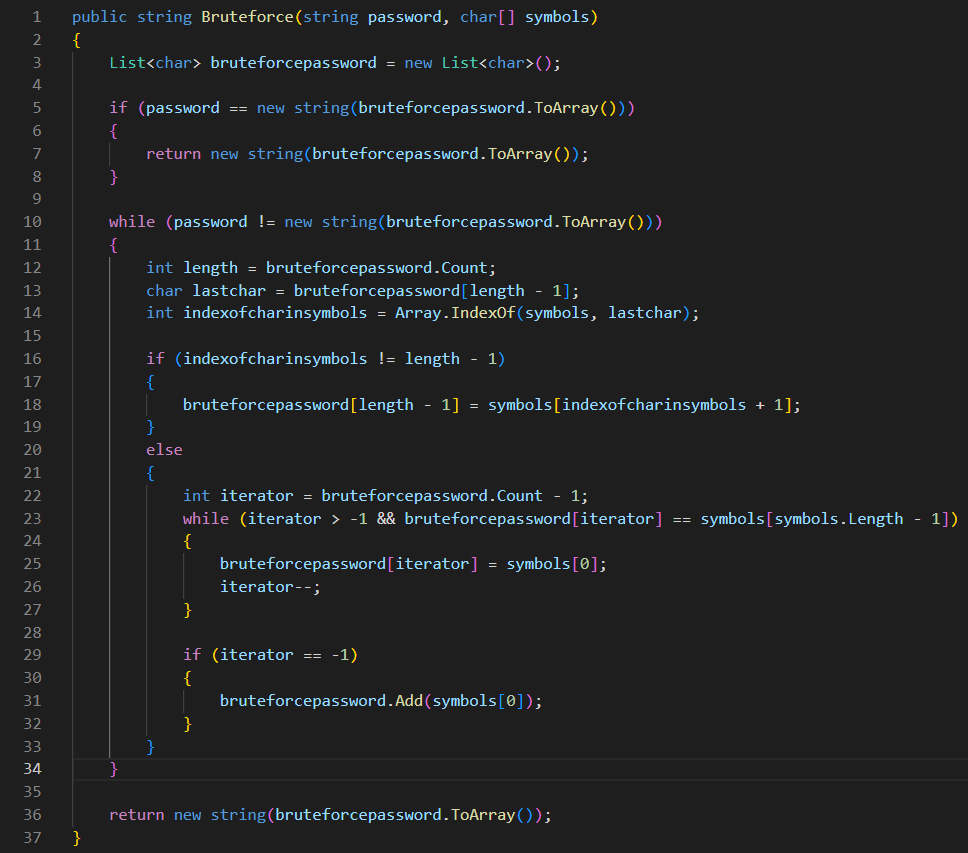
\includegraphics[width=0.7\textwidth]{Bruteforcecode.png}
     \caption[Quellcode des Brute-Force Algorithmus]{selbstgeschriebener Quellcode eines Brute-Force Algorithmus\protect\footnotemark}
     \label{Quellcode des Brute-Force Algorithmus}
  \end{figure}
In der Abbildung ist ein Beispiel Code zusehen, welcher ein Passwort anhand eines Brute-Force Algorithmuses findet. 
Der gegebene Code implementiert eine Funktion namens ``Bruteforce``  in C-Sharp.
Diese Funktion verwendet eine Brute-Force-Methode, um ein Passwort zu erraten, indem sie systematisch alle möglichen Kombinationen von Zeichen ausprobiert.
Der Funktion werden zwei Parameter übergeben: das zu erratende Passwort als Zeichenfolge und ein Array von Symbolen, aus denen die Kombinationen gebildet werden sollen.
Zu Beginn wird eine leere Liste namens ``bruteforcepassword`` erstellt. Dann wird überprüft, ob das gegebene Passwort bereits mit der aktuellen Kombination übereinstimmt. 
Wenn dies der Fall ist, wird die aktuelle Kombination als Zeichenfolge zurückgegeben.
Ansonsten wird eine Schleife gestartet, die solange läuft, bis das gegebene Passwort mit der aktuellen Kombination übereinstimmt. 
In jeder Iteration wird die Länge der aktuellen Kombination bestimmt und das letzte Zeichen abgerufen. 
Es wird der Index dieses Zeichens im Symbol-Array ermittelt.
Wenn der Index nicht gleich der Länge minus eins ist, wird das letzte Zeichen durch das nächste Zeichen im Symbol-Array ersetzt.
Wenn der Index gleich der Länge minus eins ist, bedeutet dies, dass das letzte Zeichen bereits das letzte verfügbare Symbol ist. 
In diesem Fall wird ein Iterator initialisiert, der vom Ende der aktuellen Kombination bis zum Anfang durchläuft. 
Solange das aktuelle Zeichen das letzte verfügbare Symbol ist, wird es durch das erste Symbol im Symbol-Array ersetzt. 
Wenn der Iterator den Anfang erreicht und das aktuelle Zeichen immer noch das letzte Symbol ist, wird das erste Symbol am Ende der aktuellen Kombination hinzugefügt.
Nachdem die Schleife beendet ist und das Passwort gefunden wurde, wird die aktuelle Kombination als Zeichenfolge zurückgegeben.
\subsection{Dictionary Attacks}
\subsubsection{Defintion}
Ein Dictionary-Angriff, auch als Wörterbuch-Angriff bezeichnet, ist eine Methode, um Passwörter oder Schlüssel durch systematisches Ausprobieren einer Liste häufig verwendeter Wörter, Phrasen oder Passwortkombinationen zu knacken.
Bei einem Dictionary-Angriff wird eine vordefinierte Liste, auch als Wörterbuch oder Dictionary bezeichnet, verwendet, die potenzielle Passwörter oder Schlüssel enthält. 
Diese Liste kann verschiedene Formen annehmen, wie beispielsweise eine Sammlung häufig verwendeter Wörter, bekannte Passwörter, gebräuchliche Phrasen oder Kombinationen aus Wörtern und Zahlen.
Der Angriff erfolgt, indem das Programm oder Skript die Liste der Wörter systematisch mit dem Ziel durchprobiert, das Passwort oder den Schlüssel zu finden. 
Es werden verschiedene Variationen und Kombinationen der Wörter aus dem Wörterbuch ausprobiert, einschließlich der Verwendung von Zahlen, Sonderzeichen und Groß- oder Kleinschreibung.
\subsubsection{Funktionsweise}
Die Abbildung veranschaulicht die Funktionsweise eines einfachen Dictionary-Attack-Algorithmus.
\begin{figure}[H]
    \centering
      \includegraphics[width=0.7\textwidth]{dictionary.png}
     \caption[Quellcode eines Dictionary Algorithmus]{selbstgeschriebener Quellcode eines Dictionary Algorithmus\protect\footnotemark}
     \label{Quellcode eines Dictionary Algorithmus}
  \end{figure}
  In diesem Beispielcode wird eine Methode "DictionaryAttack" implementiert, die ein Passwort und eine Liste von Wörtern als Parameter akzeptiert. 
  Der Code durchläuft anschließend jedes Wort in der Liste und vergleicht es mit dem gegebenen Passwort.
  Wenn das Passwort mit einem Wort aus der Liste übereinstimmt, wird das gefundene Wort als Ergebnis zurückgegeben. 
  Andernfalls wird null zurückgegeben, wenn keine Übereinstimmung gefunden wurde.
\subsection{Komplexität von Passwörtern}
Die Anzahl der möglichen Lösungen für ein Passwort kann durch die folgende Formel berechnet werden: Kombinationen = Zeichenanzahl \textsuperscript{Passwortlänge} \footcite[Vgl][S. 2]{ETHZürich}. 
Diese Formel ermöglicht die Untersuchung der verschiedenen Kombinationsmöglichkeiten von Passwörtern. Dabei werden die Ziffern betrachtet, die aus 10 verschiedenen Symbolen bestehen. 
Ebenso werden die Kleinbuchstaben der deutschen Sprache ohne Sonderzeichen berücksichtigt, die aus 26 Symbolen bestehen. 
Zusätzlich werden auch Kleinbuchstaben, Großbuchstaben und Ziffern betrachtet, wodurch sich eine Menge von 62 verschiedenen Symbolen ergibt.
\newpage
\begin{table}[h]
    \centering
    \begin{tabular}{ |c|c|c|c| } 
     \hline
     \textbf{Passwortlänge} & \textbf{Ziffern} & \textbf{Kleinbuchstaben} & \textbf{Kleinbuchstaben, Großbuchstaben und Ziffern}\\ 
     \hline
     1 & $10^1$ & 26 & 62 \\
     2 & $10^2$ & 676 & 3,844 \\
     3 & $10^3$ & 17,576 & 238,328 \\
     4 & $10^4$ & 456,976 & 14,776,336 \\
     5 & $10^5$ & 11,881,376 & 916,132,832 \\
     6 & $10^6$ & 308,915,776 & 56,800,235,584 \\
     7 & $10^7$ & 8,031,810,176 & 3,521,614,606,208 \\
     8 & $10^8$ & 208,827,064,576 & 218,340,105,584,896 \\
     9 & $10^9$ & 5,429,503,678,976 & 13,537,086,546,263,552 \\
     10 & $10^{10}$ & 141,167,095,653,376 & 839,299,365,868,340,224 \\
     11 & $10^{11}$ & 3,670,344,486,987,776 & 52,031,252,847,222,976,512 \\
     12 & $10^{12}$ & 95,428,956,661,682,176 & 3,226,266,762,397,899,821,824 \\
     \hline
    \end{tabular}
    \caption[Kombinationen von Passwörtern]{Kombinationsmöglichkeiten von Passwörtern}
\end{table}
Interessant ist die Passwortlänge von acht, da ein WPA2-Passwort mindestens aus acht Zeichen bestehen muss. 
Bei der Betrachtung der möglichen Kombinationen wird deutlich, dass bei Verwendung von nur Ziffern 10 Millionen Möglichkeiten existieren. 
Im Vergleich dazu gibt es mehr als das 2.000-fache an Möglichkeiten bei Verwendung von Kleinbuchstaben. 
Wenn wir die Kombination von Kleinbuchstaben, Großbuchstaben und Ziffern betrachten, ergibt sich ein Unterschied, der größer als der Faktor 1.000 ist.
\subsection{WPA 2}
WPA2 (Wi-Fi Protected Access 2) ist ein Sicherheitsprotokoll, das in Wi-Fi-Netzwerken verwendet wird, um die Vertraulichkeit und Integrität der drahtlosen Kommunikation zu gewährleisten. 
Es ist der Nachfolger von WPA und bietet eine stärkere Verschlüsselung und verbesserte Sicherheitsfunktionen.
Die Funktionsweise von WPA2 basiert auf einem Vier-Wege-Handshake, der zwischen dem Client (z. B. ein Laptop oder ein Smartphone) und dem Access Point (der drahtlosen Basisstation) stattfindet. 
Der Handshake ermöglicht es beiden Parteien, sich gegenseitig zu authentifizieren und einen gemeinsamen geheimen Sitzungsschlüssel zu etablieren, der für die Verschlüsselung des Datenverkehrs verwendet wird.
WPA2 verwendet zur Verschlüsselung des Passworts den PBKDF2 (Password-Based Key Derivation Function 2)-Algorithmus. Bei PBKDF2 handelt es sich um einen Algorithmus zur Derivation von Schlüsseln basierend auf einem Passwort.

Der Schlüssel für die Verschlüsselung setzt sich dabei aus verschiedenen Komponenten zusammen, nämlich dem Passwort selbst, dem Salt (einem zufälligen Wert), der Anzahl der Iterationen, der verwendeten Hash-Funktion und der Länge des abgeleiteten Schlüssels.
Diese Parameter werden in der Formel key = (password, salt, iterations-count, hash-function, derived-key-len) festgelegt. \footcite{PBKDF2}
\subsection{Rainbow Tables}
\subsubsection{Definition}
Die Rainbow-Tabelle, auch bekannt als Regenbogentabelle, ist eine Datenstruktur, die von Philippe Oechslin entwickelt wurde \cite{Rainbow}. 
Sie ermöglicht eine effiziente und speichersparende Suche nach der ursprünglichen Zeichenfolge, in der Regel ein Passwort, basierend auf einem gegebenen Hashwert. 
Die Rainbow-Tabelle ist eine bedeutende technologische Entwicklung im Bereich der kryptografischen Sicherheit und spielt eine wichtige Rolle bei der Entschlüsselung von Passwörtern und der Sicherheitsanalyse von Hashfunktionen.
\subsubsection{WPA2}
Im Kontext von WPA2 werden Rainbow-Tabellen vor dem Angriff auf das WPA2-Netzwerk neu generiert. 
Beim Erzeugen des Schlüssels wird folgende Formel verwendet: key = pbkdf2(Passwort, SSID, 4096, HMAC-SHA1, 256). 
Die SSID des WLANs wird als Teil des Schlüssels verwendet, um eine eindeutige Verknüpfung zwischen dem Passwort und dem Netzwerk herzustellen. 
Vor dem Angriff können mit Hilfe von Techniken wie der Dictionary-Attack oder Brute-Force viele Schlüssel-Hashwert-Paare erzeugt werden.
Im 4-Wege-Handshake, der zur Authentifizierung zwischen dem Access Point und dem Client stattfindet, wird das verhashte Passwort aufgezeichnet. 
In der dritten Nachricht des 4-Wege-Handshakes, dem EAPOL-Key, ist der PTK (Pairwise Transient Key) enthalten. Der PTK setzt sich aus dem PMK (Pairwise Master Key), zwei zufälligen Zahlen, die zuvor ausgetauscht wurden, sowie den MAC-Adressen des Benutzers und des Access Points zusammen. \footcite[VGL]{professional}
Der PMK ist das verhashte Passwort, das in der Rainbow-Tabelle gesucht werden kann. 
Wenn ein passender Hashwert in der Rainbow-Tabelle gefunden wird, bedeutet dies, dass das ursprüngliche Passwort ebenfalls gefunden wurde. 
Die Rainbow-Tabelle ermöglicht es Angreifern, auf effiziente Weise Passwörter zu entschlüsseln und somit Zugang zu einem geschützten WPA2-Netzwerk zu erlangen. 


    
    
 
